\section{Vettori Aleatori e Machine Learning}\label{sec:va_ml}

\subsection{Apprendimento Supervisionato (Supervised Learning)}

\begin{definizione}{Apprendimento Supervisionato}{def:supervised_learning}
Nell'apprendimento supervisionato, l'obiettivo è predire una o più variabili di output a partire da un insieme di variabili di input (dette predittori).
\end{definizione}

\begin{esempio}{Casi d'uso}{supervised_cases}
Alcune applicazioni pratiche includono:
\begin{itemize}
    \item Prevedere le risorse necessarie (tempo, soldi, energia) per una commessa o un progetto.
    \item Prevedere il peso corporeo di un soggetto basandosi su altre misure fisiche.
    \item Classificare il contenuto di un'immagine, assegnandola a una categoria specifica.
\end{itemize}
\end{esempio}

\begin{figure}[ht]
\centering
\begin{tikzpicture}
\begin{axis}[
    width=12cm,
    height=6cm,
    xlabel={Statura ($y$)},
    ylabel={Densità},
    xtick={168, 175},
    ytick=\empty,
    axis y line=left,
    axis x line=bottom,
    enlarge x limits=0.1,
    samples=100,
    domain=140:210,
]

% Parametri delle distribuzioni
\def\muM{175} % Media maschi
\def\muF{168} % Media femmine
\def\sigmaVal{7} % Deviazione standard

% Distribuzione condizionata per X=0 (maschi)
\addplot[blue, thick] {gauss(x, \muM, \sigmaVal)};
\node[above, blue] at (axis cs:178, {gauss(175, \muM, \sigmaVal)}) {\(f_{Y|X}(y|X=0)\)};

% Distribuzione condizionata per X=1 (femmine)
\addplot[violet, thick] {gauss(x, \muF, \sigmaVal)};
\node[above, violet] at (axis cs:165, {gauss(168, \muF, \sigmaVal)}) {\(f_{Y|X}(y|X=1)\)};

% Distribuzione marginale di Y (curva verde)
\addplot[green!60!black, thick, dashed] {0.5*gauss(x, \muM, \sigmaVal) + 0.5*gauss(x, \muF, \sigmaVal)};

% Linee tratteggiate per indicare le medie
\draw[dashed] (axis cs:\muM, 0) -- (axis cs:\muM, {gauss(\muM, \muM, \sigmaVal)});
\draw[dashed] (axis cs:\muF, 0) -- (axis cs:\muF, {gauss(\muF, \muF, \sigmaVal)});

\end{axis}
\end{tikzpicture}
\caption{Illustrazione della distribuzione della statura \(Y\) condizionata dal sesso \(X\). Le curve continue sono le densità condizionate per maschi (\(\mu=175\)) e femmine (\(\mu=168\)). La curva tratteggiata è la densità marginale di \(Y\).}
\label{fig:distribuzione-mista-gauss}
\end{figure}

Il concetto fondamentale è imparare la relazione che lega l'input \(X\) all'output \(Y\). Ad esempio, si può modellare la relazione tra il sesso di una persona (\(X\)) e la sua statura (\(Y\)). In questo caso, \(X\) è una variabile discreta (es. 0 per maschio, 1 for femmina) e \(Y\) è una variabile continua. Dopo aver appreso il modello, per un dato input si ottiene la distribuzione dell'output. Per \(X=0\) (maschio), la statura \(Y\) potrebbe seguire una distribuzione \(\mathcal{N}(175, 7^2)\), mentre per \(X=1\) (femmina), \(Y \sim \mathcal{N}(168, 7^2)\). Questa relazione è descritta dalla distribuzione condizionata \(f_{Y|X}(y|x)\).

\begin{nota}{Indipendenza delle Variabili}{nota:indipendenza_predizione}
Se una variabile di input non ha dipendenza con la variabile di output (es. colore degli occhi rispetto alla statura), la predizione per l'output \(Y\) non sarà condizionata da tale input, ma risulterà in una distribuzione mista (mixture).
\end{nota}


\subsection{Apprendimento non Supervisionato (Unsupervised Learning)}

\begin{definizione}{Apprendimento non Supervisionato}{def:unsupervised_learning}
Nell'apprendimento non supervisionato, non ci sono variabili di output predefinite. L'obiettivo è esplorare i dati per capire la loro distribuzione multivariata e scoprire pattern o strutture intrinseche.
\end{definizione}

\begin{esempio}{Clusterizzazione di Cellule}{unsupervised_cases}
Un'applicazione tipica è la clusterizzazione di dati biologici. Ad esempio, partendo da un dataset dove le righe sono cellule e le colonne sono l'espressione di migliaia di geni, l'obiettivo è:
\begin{itemize}
    \item Trovare le relazioni tra le variabili (i geni).
    \item Scoprire come si raggruppano le cellule in base a questi pattern.
    \item Cercare di identificare e dare un significato a questi cluster.
\end{itemize}
\end{esempio}

\subsection{La Matrice di Covarianza}

\begin{definizione}{Matrice di Covarianza}{def:cov_matrix}
Dato un vettore aleatorio \(X = (X_1, \dots, X_m)\), la sua matrice di covarianza, indicata con \(\Sigma\) o \(C(X)\), è una matrice \(m \times m\) i cui elementi rappresentano la covarianza tra le componenti del vettore.
L'elemento \((i, j)\) della matrice è definito come:
\[
\Sigma_{ij} := \text{Cov}(X_i, X_j)
\]

\end{definizione}

\begin{proposizione}{Proprietà della Matrice di Covarianza}{prop:cov_matrix_props}
\begin{itemize}
    \item È una matrice \textbf{simmetrica}, poiché \(\text{Cov}(X_i, X_j) = \text{Cov}(X_j, X_i)\).
    \item Sulla diagonale principale si trovano le \textbf{varianze} delle singole componenti, \(\Sigma_{ii} = \text{Var}(X_i)\), che sono sempre non negative.
    \item Se le componenti \(X_1, \dots, X_m\) sono \textbf{indipendenti} tra loro, la matrice di covarianza è \textbf{diagonale}, in quanto tutte le covarianze tra variabili diverse sono nulle.
\end{itemize}
\end{proposizione}

\begin{nota}{Ripasso sulla Covarianza}{nota:cov_recall}
L'operatore covarianza \(\text{Cov}(\cdot, \cdot)\) è bilineare e ha le seguenti proprietà:
\begin{itemize}
    \item \(\text{Cov}(X, X) = \text{Var}(X)\).
    \item \(\text{Cov}(X, Y) = \text{Cov}(Y, X)\).
    \item Se \(X\) e \(Y\) sono indipendenti, allora \(\text{Cov}(X, Y) = 0\).
    \item La covarianza con una costante è zero: \(\text{Cov}(X, \text{cost}) = 0\).
\end{itemize}
\end{nota}

\section{Trasformazioni Lineari di Vettori Aleatori}\label{sec:trasf_lineari_va}

\subsection{Definizione}
Una trasformazione lineare è una funzione che mappa un vettore da uno spazio a un altro tramite operazioni di rotazione, scalatura e traslazione.

\begin{definizione}{Trasformazione Lineare di un Vettore Aleatorio}{def:trasf_lineare_vett}
Dato un vettore aleatorio \(X \in \mathbb{R}^m\), una trasformazione lineare \(g: \mathbb{R}^m \to \mathbb{R}^k\) è definita come:
\[
Y = g(X) = \alpha + BX
\]
dove \(\alpha \in \mathbb{R}^k\) è un vettore di costanti (traslazione) e \(B \in M_{k,m}\) è una matrice di costanti (rotazione, scalatura, deformazione).
\end{definizione}

\begin{nota}{Effetto Geometrico}{nota:effetto_trasformazione}
L'effetto di una trasformazione lineare sulla distribuzione di un vettore aleatorio può essere visualizzato geometricamente:
\begin{itemize}
    \item Il vettore \(\alpha\) causa una \textbf{traslazione} della distribuzione nello spazio.
    \item La matrice \(B\) applica una \textbf{rotazione} e una \textbf{deformazione}. Se la matrice \(B\) è diagonale, l'effetto è una semplice scalatura indipendente su ciascuna componente.
\end{itemize}
\end{nota}

\subsection{Trasformazione di Media e Covarianza}
Quando si applica una trasformazione lineare a un vettore aleatorio, anche la sua media e la sua matrice di covarianza si trasformano secondo regole precise.

\begin{proposizione}{Trasformazione della Media}{prop:media_trasformata}
Sia \(X\) un vettore aleatorio con media \(\mu_X = E(X)\). La media del vettore trasformato \(Y = \alpha + BX\) è:
\[
\mu_Y = \alpha + B\mu_X
\]
\end{proposizione}
\begin{dimostrazione}{}{}
La dimostrazione segue dalla definizione di prodotto matrice-vettore e dalla linearità del valore atteso applicata a ogni componente.

Consideriamo la componente i-esima del vettore \(Y\):
\[
Y_i = \alpha_i + [BX]_i = \alpha_i + \sum_{j=1}^m B_{ij} X_j
\]
Calcoliamo il valore atteso di \(Y_i\) per ottenere la componente i-esima della media \(\mu_Y\):
\begin{align*}
    [\mu_Y]_i &= E[Y_i] \\
    &= E\left[ \alpha_i + \sum_{j=1}^m B_{ij} X_j \right] \\
    &= E[\alpha_i] + E\left[ \sum_{j=1}^m B_{ij} X_j \right] &\quad \text{(per linearità di $E$)} \\
    &= \alpha_i + \sum_{j=1}^m B_{ij} E[X_j] &\quad \text{($B_{ij}$ costanti)} \\
    &= \alpha_i + \sum_{j=1}^m B_{ij} [\mu_X]_j
\end{align*}
L'ultima espressione, \( \alpha_i + \sum_{j=1}^m B_{ij} [\mu_X]_j \), è per definizione la componente i-esima del vettore \( \alpha + B\mu_X \).
Poiché \( [\mu_Y]_i = [\alpha + B\mu_X]_i \) vale per ogni componente \(i\), l'uguaglianza tra i vettori è dimostrata.
\end{dimostrazione}


\begin{proposizione}{Trasformazione della Matrice di Covarianza}{cov_trasformata}
Sia \(X\) un vettore aleatorio con matrice di covarianza \(\Sigma_X = C(X)\). La matrice di covarianza del vettore trasformato \(Y = \alpha + BX\) è:
\[
\Sigma_Y = B \Sigma_X B^\mathsf{T}
\]
\end{proposizione}
\begin{dimostrazione}{}{}
Il termine di traslazione \(\alpha\) non influenza la covarianza. Calcoliamo l'elemento \((i, j)\) della matrice \(\Sigma_Y\), ricordando che \(Y_i = \alpha_i + \sum_k B_{ik}X_k\):
\begin{align*}
    [\Sigma_Y]_{ij} &= \text{Cov}(Y_i, Y_j) = \text{Cov}\left(\alpha_i + \sum_k B_{ik}X_k, \alpha_j + \sum_h B_{jh}X_h\right) \\
    &= \text{Cov}\left(\sum_k B_{ik}X_k, \sum_h B_{jh}X_h\right) \quad \text{(per la bilinearità della covarianza)} \\
    &= \sum_k \sum_h B_{ik} B_{jh} \text{Cov}(X_k, X_h) \\
    &= \sum_k \sum_h B_{ik} [\Sigma_X]_{kh} B_{jh}
\end{align*}
Questa espressione corrisponde esattamente all'elemento \((i, j)\) del prodotto matriciale \(B \Sigma_X B^\mathsf{T}\).
\end{dimostrazione}

\subsection{Il Coefficiente di Correlazione Lineare}

\begin{definizione}{Coefficiente di Correlazione Lineare}{def:corr_coeff}
Date due variabili aleatorie \(X\) e \(Y\) con varianze finite e non nulle, il loro coefficiente di correlazione lineare (di Pearson), denotato con \(\rho(X,Y)\), è definito come:
\[
\rho(X,Y) := \frac{\text{Cov}(X,Y)}{\sqrt{\text{Var}(X)\text{Var}(Y)}}
\]
\end{definizione}

\begin{nota}{Proprietà della Correlazione}{nota:corr_props}
\begin{itemize}
    \item È una misura adimensionale normalizzata della covarianza, con valori sempre compresi nell'intervallo \([-1, 1]\).
    \item Misura la forza e la direzione della \textbf{relazione lineare} tra due variabili.
    \item Un valore vicino a \(+1\) indica una forte correlazione positiva, vicino a \(-1\) una forte correlazione negativa, e vicino a \(0\) un'assenza di correlazione lineare.
\end{itemize}
\end{nota}

\subsection{Trasformazioni Lineari Frequenti}
Alcune trasformazioni lineari sono usate così spesso nel pre-processing dei dati da meritare una menzione speciale.

\subsubsection{Centrare il Vettore}
L'obiettivo di questa trasformazione è spostare la distribuzione dei dati in modo che la sua media sia il vettore nullo.
\begin{itemize}
    \item \textbf{Trasformazione:} Si sottrae il vettore delle medie \(\mu_X\) dal vettore aleatorio \(X\).
    \[ Y = X - \mu_X \]
    \item \textbf{Forma Matriciale:} Corrisponde a \(Y = \alpha + BX\) con \(\alpha = -\mu_X\) e \(B=I\) (matrice identità).
    \item \textbf{Risultato:} La nuova media è nulla, mentre la matrice di covarianza rimane invariata.
    \[ \mu_Y = E(Y) = 0, \quad \Sigma_Y = C(Y) = \Sigma_X \]
    \item \textbf{A livello di campione:} Questa operazione equivale a sottrarre da ogni dato la media della sua colonna: \(Y_{ij} = X_{ij} - \bar{X}_j\).
\end{itemize}

\begin{figure}[H]
    \centering
    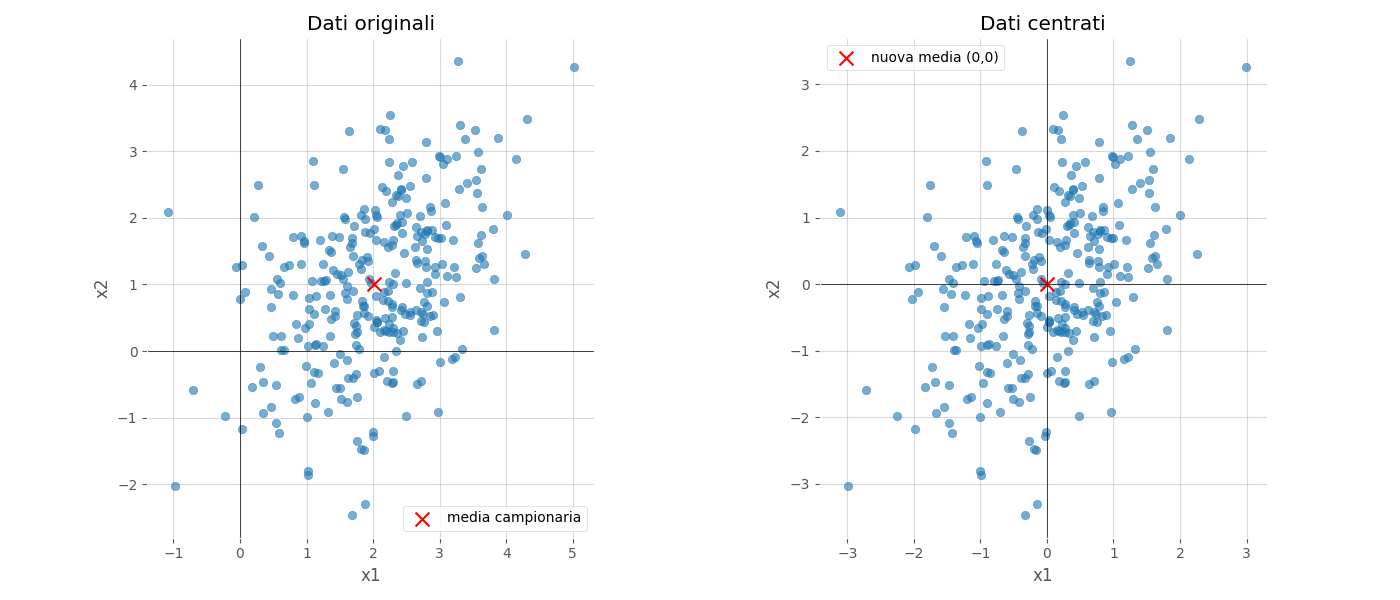
\includegraphics[width=\textwidth]{images/th_07_09/centering_transformation.png}
    \caption{Esempio di centratura di un vettore aleatorio bidimensionale. La distribuzione originale (a sinistra) viene traslata in modo che la sua media coincida con l'origine (a destra).}
    \label{fig:centering_transformation}
\end{figure}

\subsubsection{Standardizzare le Varianze}
L'obiettivo è scalare le componenti del vettore in modo che abbiano tutte
varianza unitaria (pari a 1).
\begin{itemize}
    \item \textbf{Trasformazione:} Si divide ogni componente \(X_i\) per la sua
    deviazione standard \(\text{std}(X_i)\).
    \[ Y_i = \frac{X_i}{\text{std}(X_i)} \]
    \item \textbf{Forma Matriciale:} Corrisponde a \(Y = BX\) dove \(B\) è una
    matrice diagonale contenente le inverse delle deviazioni standard:
    \[ B = \text{diag}(\text{std}(X_1)^{-1}, \dots, \text{std}(X_m)^{-1}) \]
\item \textbf{Risultato:} La matrice di covarianza del vettore trasformato \(Y\)
diventa la \textbf{matrice di correlazione} del vettore originale \(X\).
L'elemento \((i,j)\) di \(C(Y)\) è:
\[
    [C(Y)]_{ij} = \text{Cov}\left(\frac{X_i}{\text{std}(X_i)}, \frac{X_j}{\text{std}(X_j)}\right)
    \stackrel{\text{\tiny(per bilinearità della Cov)}}{=} \frac{\text{Cov}(X_i, X_j)}{\text{std}(X_i)\text{std}(X_j)}
    = \rho(X_i, X_j)
\]
\end{itemize}

\begin{figure}[H]
    \centering
    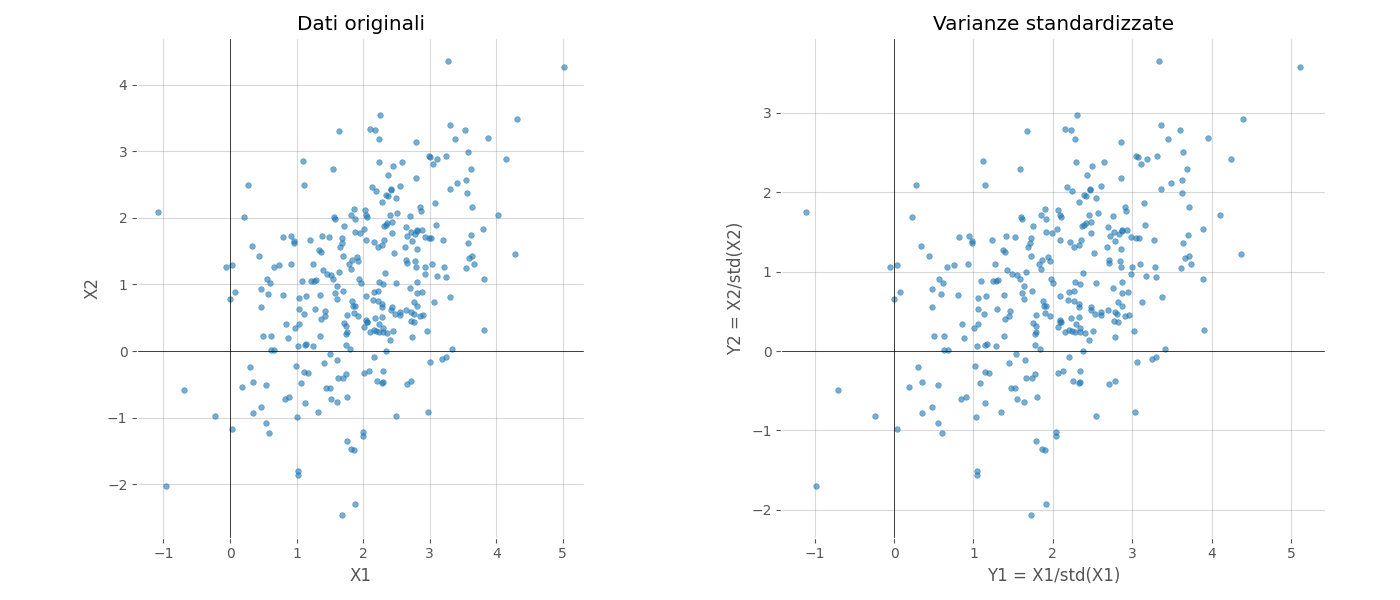
\includegraphics[width=\textwidth]{images/th_07_09/standardize_variances.png}
    \caption{Esempio di standardizzazione delle varianze di un vettore aleatorio bidimensionale. La distribuzione originale (a sinistra) viene trasformata in modo che le sue varianze siano tutte pari a 1 (a destra).}
    \label{fig:standardize_variances}
\end{figure}

\paragraph{Standardizzazione Completa (Z-score)}
Questa trasformazione combina le due precedenti per ottenere un vettore le cui
componenti hanno media 0 e varianza 1.
\begin{itemize}
    \item \textbf{Trasformazione:} È l'operazione nota come calcolo dello
    Z-score.
    \[ Y_i = \frac{X_i - E(X_i)}{\text{std}(X_i)} \]
    \item \textbf{Forma Matriciale:} Si applicano in ordine la centratura e la
    standardizzazione della varianza.
    \[ Y = \text{diag}(\text{std}(X)^{-1}) (X - \mu_X) \]
    \item \textbf{Risultato:} Il vettore trasformato \(Y\) ha media nulla e la
    sua matrice di covarianza coincide con la matrice di correlazione di \(X\).
    \[ \mu_Y = 0, \quad \Sigma_Y = \rho(X) \]
\end{itemize}

\begin{figure}[H]
    \centering
    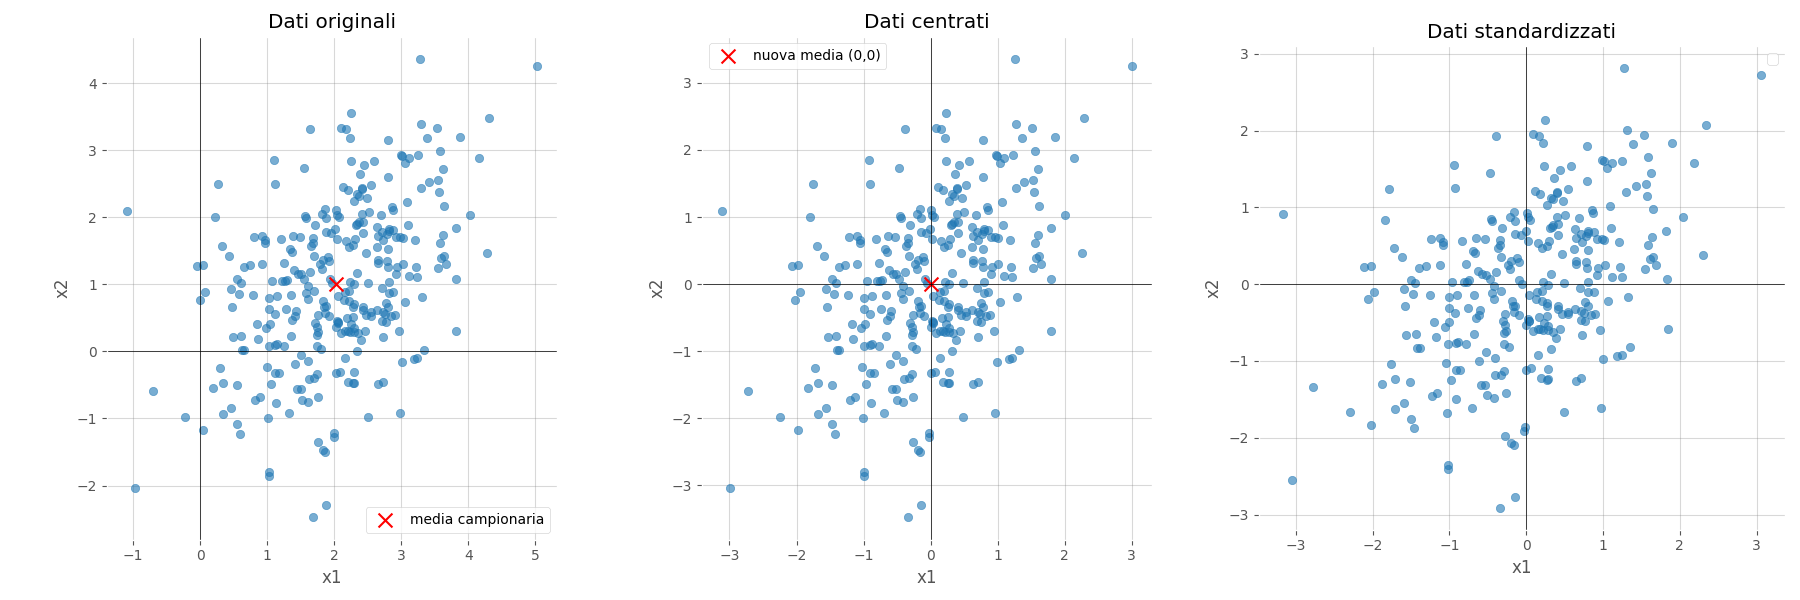
\includegraphics[width=\textwidth]{images/th_07_09/z_transformation.png}
    \caption{Esempio di standardizzazione (Z-score) di un vettore aleatorio bidimensionale. La distribuzione originale (a sinistra) viene trasformata in modo che le sue componenti abbiano media 0 (in centro) e varianza 1 (a destra).}
    \label{fig:z_transformation}
\end{figure}